\section{Data}
The data for this case study is two-fold. First, the random variable of
interest is the total daily revenue of a restaurant chain - OLIOLI - and is a
sum of the revenue generated for each transaction retrieved and formatted via
the Point of Sale systems in each store. The number of stores open on a given
day was also collected. Second, for each day, collected and forecasted weather
data is sourced from Visual Crossing - a leading weather data provider. The
data set used for this project is populated with revenue figures and weather
metrics for each day from the 1st of January 2020 to the 23rd of April 2023.
The data set contains 1209 observations, each representing a day, and Figure
\ref{fig:variables} presents the variables that were collected.
\begin{figure}[h!]
    \begin{subfigure}{0.5\textwidth}
      \centering
      \caption{Variable Source}
      \label{fig:vars1}
      \begin{tabular}{l}
          \toprule 
          \textbf{Weather variables} \\
          \quad\textit{Temperature} \\
          \quad\textit{Precipitation} \\
          \quad\textit{Wind speed} \\
          \quad\textit{Cloud cover} \\
          \quad\textit{Humidity} \\[0.3em]
          \textbf{Temporal variables} \\
          \quad\textit{Day of week} \\
          \quad\textit{Day of month} \\
          \quad\textit{Month} \\
          \quad\textit{Year} \\[0.3em]
          \textbf{Financial variables} \\
          \quad\textit{Revenue} \\
          \quad\textit{Daily revenue difference} \\
          \quad\textit{Number of stores open} \\[0.3em]
          \bottomrule
      \end{tabular}
    \end{subfigure}%
    \begin{subfigure}{0.5\textwidth}
      \centering
      \caption{Variables in Model}
      \label{fig:vars2}
      \begin{tabular}{l}
          \toprule 
          \textbf{Continuous variables} \\
          \quad\textit{Temperature} \\
          \quad\textit{Wind speed} \\
          \quad\textit{Cloud cover} \\
          \quad\textit{Humidity} \\
          \textbf{Index variables} \\
          \quad\textit{Precipitation} \\
          \quad\textit{Day of week} \\
          \quad\textit{Day of month} \\
          \quad\textit{Month} \\
          \quad\textit{Year} \\
          \quad\textit{Number of stores open} \\[0.3em]
          \textbf{Target variables} \\
          \quad\textit{Daily revenue} \\
          \quad\textit{Daily revenue difference} \\[0.3em]
          \bottomrule
      \end{tabular}
    \end{subfigure}
    \caption{Overview of the variables used in the project. Subfigure (a) categorises the variables according to their sources: 'Weather variables' comprise meteorological measures such as daily maximum temperature, total precipitation, average wind speed, cloud cover, and humidity for the day; 'Temporal variables' include calendar-based measures such as day of the week, day of the month, month, and year; 'Financial variables' encompass monetary and operational measures, such as daily revenue, daily revenue difference from the previous day, and the number of stores open. Subfigure (b) re-categorises these variables based on their role and nature in the model: 'Continuous variables' are variables that can take any value within a certain range; 'Index variables' are discrete or categorical variables, including precipitation (which is classified in different intensity categories); 'Target variables' are the dependent variables to be predicted or explained by the model, which include daily revenue and daily revenue difference.}
    \label{fig:variables}
\end{figure}

\subsection{Missing Values}
\label{subsec:missing-values}

All values in the data below a threshold were deemed invalid; due to unique
circumstances like national holidays, COVID, and shop closures. In order to
fix this, interpolation was used to replace these numbers with the mean of data
from a timeframe that included seven days before and seven days after the
problematic value.
This method ensured that the data was holistic and reliable while maintaining
the general structure and relationships between the variables. 
Furthermore, this rolling window captures any potential trends or patterns, and
the replacement numbers are consistent with the surrounding data.

Machine learning algorithms or more complex imputation methods like K-nearest
neighbours imputation are other options for handling missing variables
\cite{knn}. However, the interpolation approach used was considered appropriate
for this dataset and the objective; hence these alternatives were not pursued.

\subsection{Standardisation}

Standardisation can be an important preprocessing step in Bayesian modelling,
as it assures that variables are on a comparable scale, enabling more efficient
sampling and resulting in a more stable posterior \cite{gelman2013philosophy}.
In his paper \cite{gelman2004parameterization}, Gelman demonstrates how
reparameterisation, including standardisation, can enhance the efficiency of
the sampling process in Bayesian models \cite{gelman2004parameterization}.
Continuous variables are normalised by scaling them to have a mean of 0 and a
standard deviation of 1:
\begin{equation}
  x_{s} = \frac{x - \mu_x}{\sigma_x}
\end{equation}
The impact of extreme values in the target variable can also be reduced by
standardisation. The same formula is applied to normalise the target variable. 

Another critical point is the consistency of this standardisation. Any new data
collected and processed must be standardised with the same statistical metrics
as the rest of the data to ensure accurate and coherent inference and
prediction. This was achieved by storing each variable's mean and standard
deviation in the data set and applying the standardisation formula to new data
using these values. The reverse of the standardisation formula is applied, to
unstandardise the data using the stored mean and standard deviation. 
\begin{equation}
  x = x_{s} \cdot \sigma_x + \mu_x
\end{equation}
Revenue was also standardised to ensure data privacy and confidentiality, and
all subsequent references to revenue pertain to this standardised metric. While
the distribution of the data remains unchanged, this approach does impact the
interpretability of the results. Standardised revenue values are not
directly comparable to original revenue figures, and measures of error and
uncertainty are presented in a different context. Guidelines will be defined to
address this, referring to the standardised revenue and the company's
operational demands. To provide genuine utility, revenue predictions should
fall within 0.5 standardised revenue units of the true revenue on a given day.
As a goal, the model should be able to predict revenue within 0.3 standardised
revenue units of the true revenue on a given day. Given that sampling from a
Bayesian model's posterior predictive distribution yields a distribution of
possible outcomes, the model should be able to provide a 95\% predictive
interval that contains the true value in most forecasting cases. Specifically,
the predictive interval should be narrow enough to be useful for
decision-making purposes, yet wide enough to capture the inherent uncertainty
in the revenue prediction to ensure that the predictions are reliable and
actionable.

\subsection{Stationarity}
The nature of the problem introduces some caveats which need to be addressed in
the data. Many stores contribute to revenue generation, and over the
time-period studied, the number of stores increased from seven to fifteen. As a
company grows and expands over time, the natural and, for the company, the
ideal trend for the revenue to follow is upward. This means that the underlying
data-generating process changes - impacted by the number of stores open at a
given time, the current season and the perceived recognition and popularity of
the company, to name a few factors. In some cases, the goal is precisely to
model this trend, but doing so demands certainty in isolating the exact
variables that impact the trend. In practice, this was not feasible, and some
of the models developed in this paper make some assumptions about the
underlying data-generating process. One of these is the assumption of
stationarity, which states that the statistical properties of the data remain
constant over time. The intent is to model the data as a function of time
rather than a function of time and other variables, avoiding the modelling of
spurious correlations between variables and permitting the modelling of the
data as a time series, which is a common approach to forecasting
\cite{time-series1}.


\subsubsection{Methods for Resolving Non-stationarity}

Several strategies exist to address the issue of non-stationarity. One such
method involves incorporating the number of open stores as a variable. This
approach could help the model capture the cause of the increase in the mean of
the underlying data-generating process. While it is a valid option and has been
implemented, it remains uncertain if the number of stores solely influences the
mean of the data over time. The implications of this method will be discussed
further.

Another strategy to manage non-stationarity is detrending the data. Identifying
and removing underlying trends from the data can help mitigate the impact of
seasonality and long-term trends. This process could also enhance the
visibility of cyclical patterns and make it simpler to spot patterns and
linkages in the data, leading to more accurate forecasts.

An alternative option is to model not the total revenue itself but the
difference in revenue between each day and the preceding day, to remove the
linear trend. This process, known as differencing, is valuable because the
$n^{th}$ order difference of a non-stationary series is not necessarily
non-stationary.

Moreover, it is worth noting that Bayesian models offer a robust framework for
hierarchically modelling data. Therefore, it could be equally valid to model
the problem in this way. Considering the total revenue as a sum of the revenue
generated by each store, one of the benefits of this approach is that it
eliminates this specific aspect of non-stationarity from the problem. However,
this approach would require a more rigorous data processing and modelling
process, which was considered out of the scope of this project.

\subsubsection{Testing Data for Stationarity}
The test for stationarity performed was the Augmented Dickey-Fuller test. The
test's null hypothesis is that the data is non-stationary, and we then check
for the presence of a unit root \cite{adf}. A time series with a unit root
indicates that the process that produced the data followed a random walk rather
than being stationary due to the series' heavy reliance on its
historical values influencing the trends to drift over time \cite{adf}.
Implementing the test with the Python library \texttt{statsmodels} is simple,
the results of which can be seen in Table \ref{tab:adf_og}. 
\begin{table}[h]
\centering
\caption{ADF Results - Original Data}
\label{tab:adf_og}
\begin{tabular}{@{} >{\arraybackslash}l r @{}}
\toprule
\textbf{Test Statistic} & -2.1179 \\ \addlinespace[0.1em]
\textbf{P-Value} & 0.2374 \\ \addlinespace[0.1em]
\textbf{Critical Values} & \\ 
\ \ \ \ 1\% & -3.4359 \\ 
\ \ \ \ 5\% & -2.8640 \\ 
\ \ \ \ 10\% & -2.5681 \\ \addlinespace[0.1em]
\textbf{Information Criterion} & 1609.6593 \\ 
\bottomrule
\end{tabular}
\end{table}

Since the test statistic is greater than the critical values at all
significance levels, the null hypothesis that the time series has a unit root
can not be rejected (i.e. the data is non-stationary). This conclusion is
further supported by the p-value of 0.2374, greater than the standard
scientific threshold of 0.05.
\begin{table}[h]
\centering
\caption{ADF Results - First Difference}
\label{tab:adf_dif}
\begin{tabular}{@{} >{\arraybackslash}l r @{}}
\toprule
\textbf{Test Statistic} & -10.5442 \\ \addlinespace[0.1em]
\textbf{P-Value} & 8.4946e-19 \\ \addlinespace[0.1em]
\textbf{Critical Values} & \\ 
\ \ \ \ 1\% & -3.4359 \\ 
\ \ \ \ 5\% & -2.8640 \\ 
\ \ \ \ 10\% & -2.5681 \\ \addlinespace[0.1em]
\textbf{Information Criterion} & 1611.8563 \\ 
\bottomrule
\end{tabular}
\end{table}

Exploring the differencing technique mentioned above, Table \ref{tab:adf_dif}
depicts the test results after taking the first difference of the daily
revenue data. The test statistic is less than the critical values at all
significance levels, and the p-value is now less than 0.05. This indicates that
we can reject the null hypothesis that the time series has a unit root and
conclude that the first difference is stationary.
\begin{figure}[h]
\centering
\begin{subfigure}[b]{0.49\textwidth}
\centering
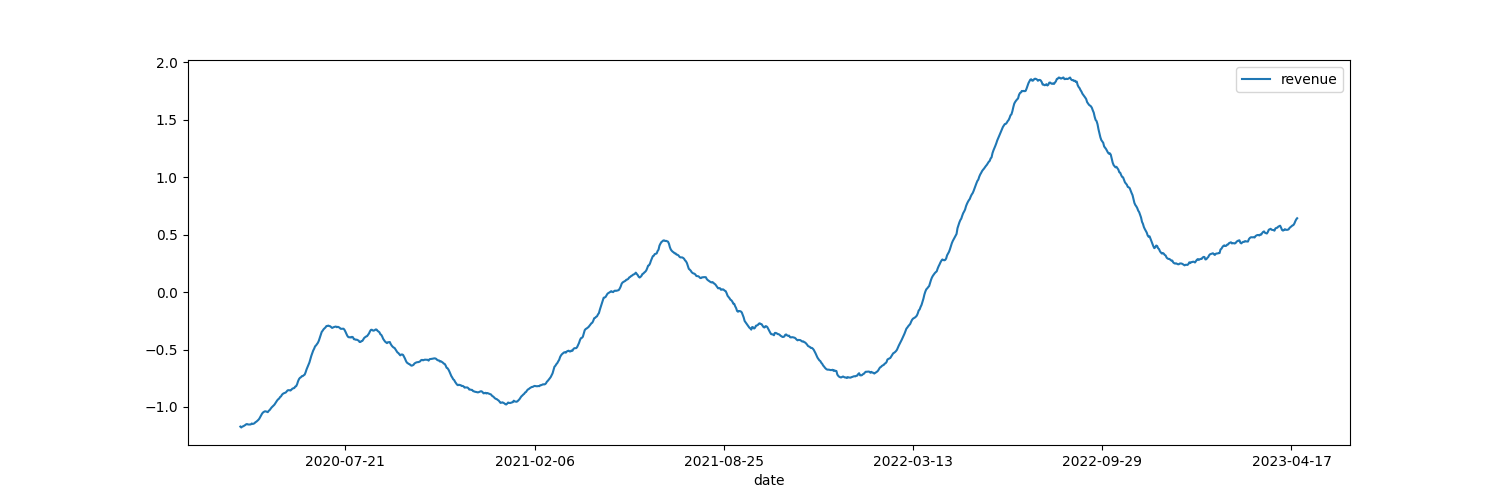
\includegraphics[width=\textwidth]{/Users/louisbrandt/itu/6/bachelor/preprocessing/plots/rolling_mean_revenue_over_time.png}
\caption{Rolling mean of revenue over time}
\label{fig:rolling_revenue_mean}
\end{subfigure}
\hfill
\begin{subfigure}[b]{0.49\textwidth}
\centering
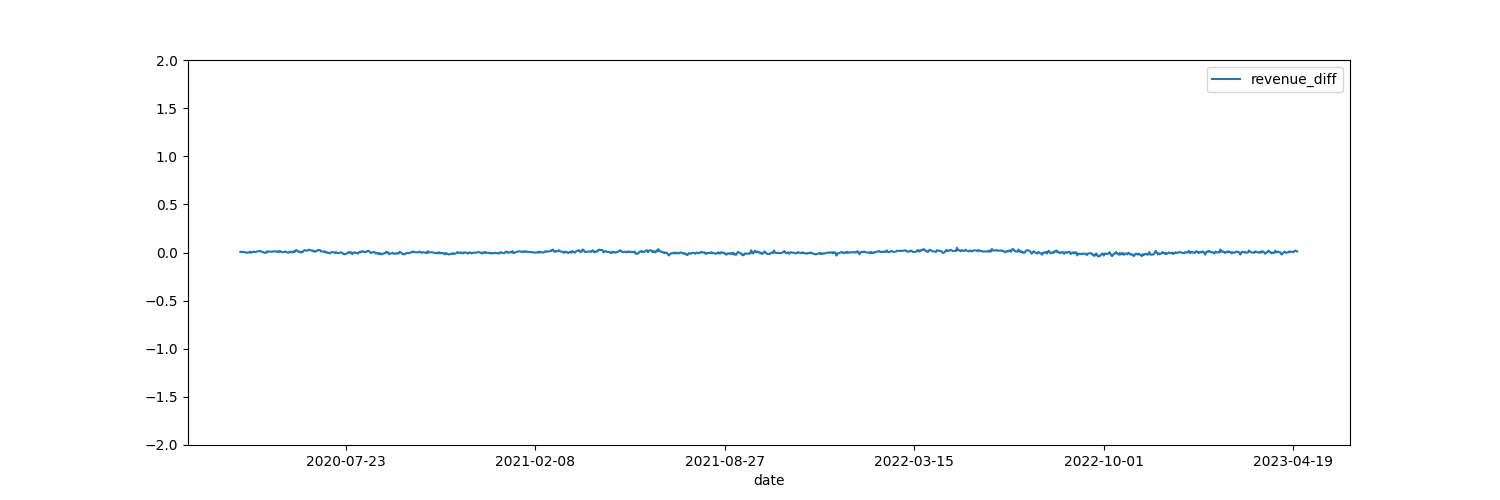
\includegraphics[width=\textwidth]{/Users/louisbrandt/itu/6/bachelor/preprocessing/plots/rolling_mean_revenue_diff_over_time.png}
\caption{Rolling mean of first revenue difference over time}
\label{fig:rolling_revenue_diff}
\end{subfigure}
\caption{Comparison of rolling mean of revenue and its first difference over time}
\label{fig:stationarity}
\end{figure}

This is further supported by the plots of the data, which can be seen in the
Figure \ref{fig:stationarity}. The original data shows an upward trend, which
is removed by taking the first difference. The first difference also shows a
more consistent variance over time, which is another requirement for
stationarity.
By modelling the first difference of the revenue instead of the revenue, it is
possible to fulfil the stationarity requirement when needed.

\subsection{Correlation Analysis}

This section examines the relationships between the different variables and the
target variable, revenue, through correlation analysis. Table
\ref{tab:correlation-numeric} presents the continuous predictors' Pearson Correlation Coefficients
(PCC), providing insights into potential linear relationships with the target
variable. These predictors include temperature, humidity, wind speed, and cloud
cover. Table \ref{tab:correlation-categorical} displays Kendall's Tau
coefficients for the categorical predictors. As a non-parametric measure,
Kendall's Tau offers insights into rank correlations between these predictors
and the target variable. The variables considered are precipitation, number of
open stores (n\_stores), day of the week (dow), day of the month (day), month,
and year. This correlation analysis paves the way for a preliminary
understanding of how each predictor might be related to the target variable.
Further visualisation can be found in the Appendix \ref{fig:corr_analysis}.
\begin{figure}[h]
  \centering
  \begin{subfigure}[b]{0.45\textwidth}
    \centering
    \caption{PCC for continuous predictors}
    \label{tab:correlation-numeric}
    \begin{tabular}{@{} >{\arraybackslash}l r @{}}
    \textbf{Variable} & \textbf{PCC} \\ \addlinespace[0.1em]
    \toprule
    \texttt{temperature} & 0.3341 \\
    \texttt{humidity} & -0.3154 \\
    \texttt{wind\_speed} & -0.2710 \\
    \texttt{cloud\_cover} & -0.1628 \\
    \bottomrule
    \end{tabular}
  \end{subfigure}
  \begin{subfigure}[b]{0.45\textwidth}
    \centering
    \caption{Kendall's Tau for categorical predictors}
    \label{tab:correlation-categorical}
    \begin{tabular}{@{} >{\arraybackslash}l r @{}}
    \textbf{Variable} & \textbf{Tau} \\ \addlinespace[0.1em]
    \toprule
    \texttt{precipitation} & -0.1748 \\
    \texttt{n\_stores} & 0.4688 \\
    \texttt{dow} & 0.0051 \\
    \texttt{day} & -0.0333 \\
    \texttt{month} & -0.0578 \\
    \texttt{year} & 0.5059 \\
    \bottomrule
    \end{tabular}
  \end{subfigure}
\caption{Results of Correlation Analysis}
\label{tab:correlations}
\end{figure}

\subsection{Data Split}
The data split strategy employed in this study hinges on the specific research
questions to address. The primary objective is to accurately forecast
future revenues, focusing on predicting revenue over a three-week period. In
light of this, the data is partitioned into training, validation, and test
sets.
The training set, spanning from 2020-01-01 to 2023-03-12, is used to build the
model. The validation set, covering 2023-03-13 to 2023-04-02, while assisting
with some tuning, primarily serves as an additional, unseen dataset to evaluate
the model's performance. It helps ensure the model's generalisability before
the final evaluation on the test set, which ranges from 2023-04-03 to
2023-04-24. 
Employing a three-week window for validation and testing is a pragmatic choice,
as real-world financial and operational decisions often involve planning
two-to-four weeks into the future.
Even though Bayesian modelling inherently integrates all available data into the model
through the likelihood function, a data split strategy still offers value. It
provides a transparent way to assess the model's generalisability, which is
vital for practical applications. It also allows for comparing between models
on the same held-out test set, giving a consistent basis for performance
evaluation. Moreover, the data split strategy can help detect potential
overfitting in the Bayesian context by assessing the model's performance across
validation and test sets.
Implementing a data split strategy in this Bayesian study thus supports a
comprehensive evaluation of the models’ predictive accuracy on different
subsets of data. It complements Bayesian model comparison techniques, providing
a systematic approach to model evaluation.
